\section{Klasifikacija}
\label{sec:Klasifikacija}

Jedan od glavnih problema u \v{c}itavom skupu je veliki broj nedostaju\'c{}ih vrednosti za \v{z}anr. Stoga smo poku\v{s}ali da napravimo klasifikator koji \'c{}e klasifikovati instance sa nepoznatim vrednostima za \v{z}anr, treniran nad onim podacima gde su te informacije dostupne.

Prvi problem na koji smo nai\v{s}li su nestandarne vrednosti za \v{z}anr (videti poglavlje \ref{sec:Preprocesiranje}), stoga smo kori\v{s}\'c{}enjem jednostavnih transformacija izvukli slogove sa nedvosmislenom vredno\v{s}\'c{}u za \v{z}anr, a eliminisali one koji su za \v{z}anr imali vrednosti koje nisu bile od zna\v{c}aja za analizu (neki slogovi su imali vi\v{s}e razli\v{c}tih \v{z}anrova). Takodje smo neke sli\v{c}ne \v{z}anrove spojili u jedan, zarad jednostavnijeg rada (na primer \emph{jazz} i \emph{blues} se \v{c}esto pojavljuju zajedno ih ima smisla posmatrati kao jedan \v{z}anr).

Za predikciju vrednosti \v{z}anra smo koristili atribite \emph{loudness}, \emph{tempo} i \emph{mode}. Na\v{z}alost, iz njihove prostorne rasprostranjenosti se vidi da ne postoji jednostavni separator instanci raznih klasa - slika \ref{fig:ZanrKlasifikacija}.

\subsection{Klasifikacija metodom K najbli\v{z}ih suseda}
\label{subsec:knn}

Prva stvar koju smo odlu\v{c}ili da isprobamo bila je \emph{KNN} algoritam u nadi da \'c{}e male grupe pesama istog \v{z}anra lepo klasifikovati bliske instance. O\v{c}ekivano, najbolji model koji smo dobili je imao preciznost od $52.65\%$. Na slici \ref{fig:KNNgreske} se mo\v{z}e videti kako se gre\v{s}ka menjala sa razli\v{c}itim vrednostima za parametar $k$.

\begin{figure}[H]
    \centering
    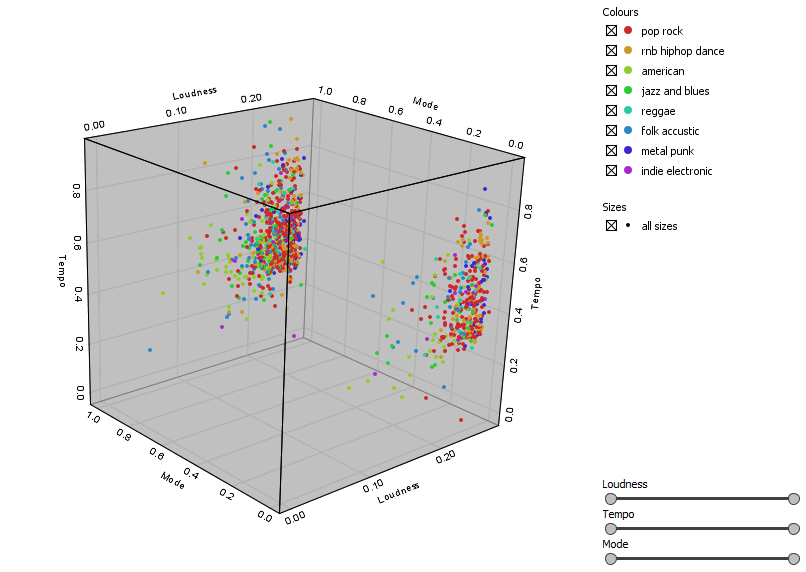
\includegraphics[scale=0.6]{resources/genre_scatter.PNG}
    \caption{3D prikaz pesama razli\v{c}itih \v{z}anrova u prostoru sa koordinatama \emph{loudness}, \emph{tempo} i \emph{mode}}
    \label{fig:ZanrKlasifikacija}
\end{figure}

\begin{figure}[H]
    \centering
    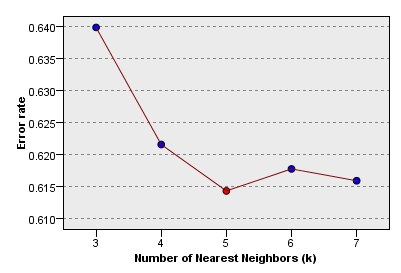
\includegraphics{resources/KNN_errors.PNG}
    \caption{Gre\v{s}ke dobijene za kreirane modele $k$ parametrom u opsegu $[3,7]$}
    \label{fig:KNNgreske}
\end{figure}

Ono \v{s}to nismo o\v{c}ekivali je jednaka va\v{z}nost atributa prilikom pravljenja klasifikatora - slika \ref{fig:KNNvaznost}. Intuicija nekako ka\v{z}e da su ja\v{c}e pesme podlo\v{z}nije da budu \v{z}anra \emph{metal}, ali rezultati su pobili tu intuiciju.

\begin{figure}[H]
    \centering
    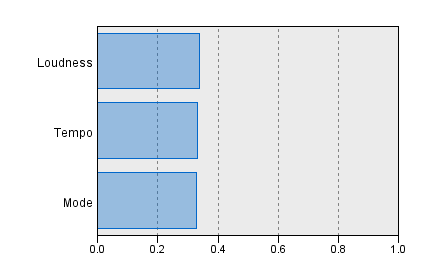
\includegraphics[scale=0.7]{resources/KNN_pred_imp.PNG}
    \caption{Va\v{z}nost atributa prilikom klasifikacije}
    \label{fig:KNNvaznost}
\end{figure}

Sled\'c{}i korak koji smo uradili bila je da isptobamo isti algoritam u alatu Knime \cite{KNIME} (prethodni zaklju\v{c}ci su dobijeni u alatu SPSS Modeler \cite{SPSS}). Ovo nam je pru\v{z}ilo mogu\'c{}nost da ru\v{c}no pridamo atributima ve\'c{}u ili manju va\v{z}nost. Iterativnim postupkom smo do\v{s}li do faktora kojima je potrebno pomno\v{z}iti vrednosti \emph{loudness} i \emph{tempo} kako bi se pove\'c{}ala preciznost klasifikatora. Ovo transformacija uti\v{c}e na izra\v{c}unavanje razli\v{c}itih euklidskih rastojanja izmedju pesama i dovela je do pobolj\v{s}anja preciznosti na $58.6\%$. Kori\v{s}\'c{}enje Menhetn rastojanja je dovelo do neznatno boljih rezultata, sa precizno\v{s}\'c{}u od $58.8\%$

Dodatno, jedno od mogu\'c{}ih unapredjenja bi bila da se u obzir uzme i atribut \emph{ModeConfidence}. Informacija o pouzdanosti vrednosti atributa koji predstavlja tonalitet pesme bi mogla da dovede do bolje klasifikacije.

\subsection{Klasifikacija stablom odlu\v{c}ivanja}
\label{subsec:stablo}
Predvidjanje \v{z}anra koriste\'c{}i stablo odlu\v{c}ivanja je takodje dalo lose rezultate. Preciznost dobijenog modela je $44.6\%$, te je gre\v{s}ka $55.4\%$. Matrica konfuzije je prikazana na slici \ref{fig:confmatrtree}.

\begin{center}
\begin{figure}[H]
    \centering
    \footnotesize
    \begin{tabular}{|c|c|c|c|c|c|c|c|c|}
        \hline
        & pop & hiphop & metal & & & jazz & accustic & indie \\
        Prediction & rock & rnb & punk & USA & reggae & blues & folk & electro \\
        & & dance & & & & & & \\
        \hline
        pop rock & 225 & 53 & 18 & 8 & 5 & 17 & 13 & 0 \\
        hiphop rnb dance & 48 & 10 & 11 & 0 & 1 & 3 & 1 & 0 \\
        metal punk & 32 & 11 & 7 & 0 & 0 & 0 & 1 & 0 \\
        american & 14 & 0 & 1 & 8 & 0 & 1 & 2 & 0 \\
        reggae & 7 & 2 & 0 & 0 & 0 & 1 & 3 & 0 \\
        jazz blues & 21 & 2 & 1 & 1 & 1 & 4 & 1 & 0 \\
        folk accustic & 18 & 4 & 2 & 1 & 1 & 3 & 2 & 0 \\
        indie electro & 6 & 1 & 0 & 1 & 0 & 0 & 0 & 0 \\
        \hline
    \end{tabular}
    \caption{Matrica konfuzije dobijena klasifikacijom stablom odlu\v{c}ivanja}
    \label{fig:confmatrtree}
\end{figure}
\end{center}

Na slici \ref{fig:tree} prikazano je dobijeno sablo odlu\v{c}ivanja. Kako vi\v{s}e od polovine pesama iz skupa pripada \v{z}anru \emph{pop rock}, a vrednosti atributa nisu dobre za klasifikaciju, stablo daje lo\v{s}e rezultate.


\begin{figure}[H]
    \centering
    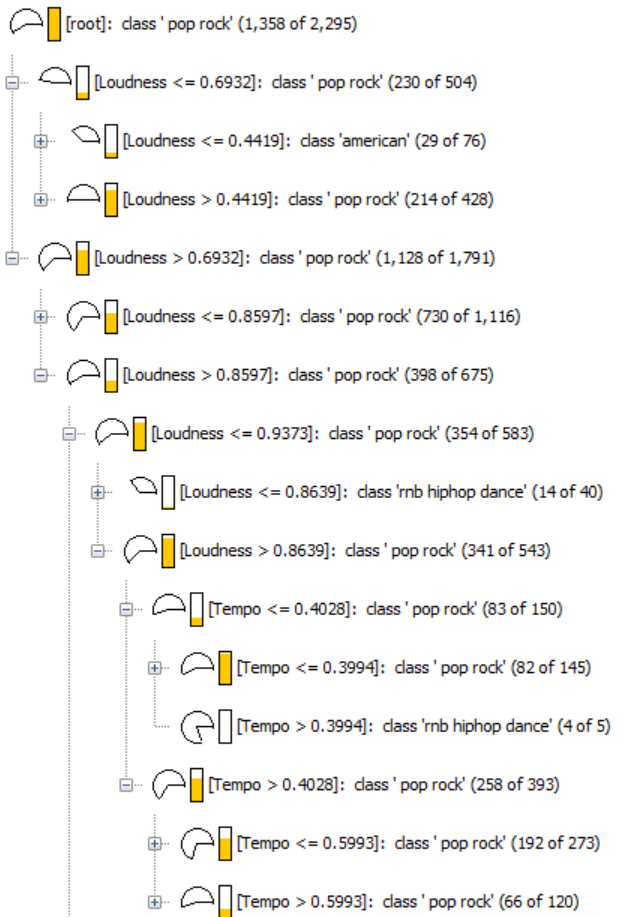
\includegraphics[scale=0.6]{resources/tree.png}
    \caption{Stablo odlu\v{c}ivanja za atrbut \v{z}anr}
    \label{fig:tree}
\end{figure}
